\chapter{ANEXO I}
\section{Conceptos y aclaraciones}

\subsection{Maven}
\label{glo:maven}
\textbf{Maven} es una herramienta de software para la gestión y construcción de proyectos Java creada por Jason van Zyl, de Sonatype, en 2002. Es similar en funcionalidad a \textbf{Apache Ant }, pero tiene un modelo de configuración de construcción más simple, basado en un formato XML. Estuvo integrado inicialmente dentro del proyecto Jakarta pero ahora ya es un proyecto de nivel superior de la Apache Software Foundation.

Maven utiliza un \textbf{POM\textit{(Project Object Model)} }para describir el proyecto de software a construir, sus dependencias de otros módulos y componentes externos, y el orden de construcción de los elementos. Viene con objetivos predefinidos para realizar ciertas tareas claramente definidas, como la compilación del código y su empaquetado. Una característica clave de Maven es que está listo para usar en red. El motor incluido en su núcleo puede dinámicamente descargar plugins de un repositorio, el mismo repositorio que provee acceso a muchas versiones de diferentes proyectos Open Source en Java, de Apache y otras organizaciones y desarrolladores. Este repositorio y su sucesor reorganizado, el repositorio Maven 2, pugnan por ser el mecanismo de facto de distribución de aplicaciones en Java, pero su adopción ha sido muy lenta. Maven provee soporte no solo para obtener archivos de su repositorio, sino también para subir artefactos al repositorio al final de la construcción de la aplicación, dejándola al acceso de todos los usuarios. Una caché local de artefactos actúa como la primera fuente para sincronizar la salida de los proyectos a un sistema local. \cite{maven}

\subsection{Gradle}
\label{glo:gradle}
\textbf{Gradle} es un sistema de automatización de construcción de código abierto que construye sobre los conceptos de Apache Ant y Apache Maven e introduce un lenguaje especifico del dominio (DSL) basado en Groovy en vez de la forma XML utilizada por Apache Maven para declarar la configuración de proyecto. \textbf{Gradle} utiliza un \textbf{DAG \textit{(Grafo Acíclico Dirigido)}} para determinar el orden en el que las tareas pueden ser ejecutadas.
\textbf{Gradle} fue diseñado para construcciones multi-proyecto las cuáles pueden crecer para ser bastante grandes, y da apoyo a construcciones incrementales determinando inteligentemente qué partes del árbol de construcción están actualizadas, de modo que cualquier tarea dependiente a aquellas partes no necesitarán ser re-ejecutada.\cite{gradle}

\subsection{Anotación Java}
\label{glo:anota}

En programación, una Anotación Java es una forma de añadir meta-datos al código fuente Java que están disponibles para la aplicación en tiempo de ejecución. Muchas veces se usa como una alternativa a la tecnología XML.

Las Anotaciones Java pueden añadirse a los elementos de programa tales como clases, métodos, campos, parámetros, variables locales, y paquetes. Al contrario que las etiquetas añadidas a la documentación Java y procesadas con las herramientas tales como XDoclet, las Anotaciones Java son completamente accesibles al programador, mientras que el software se ejecuta, usando reflexión.

\subsection{ERP}
\label{glo:erp}

El término ERP se refiere a Enterprise Resource Planning, que significa sistema de planificación de recursos empresariales. Estos programas se hacen cargo de distintas operaciones internas de una empresa, desde producción a distribución o incluso recursos humanos.

Además, los ERP ofrecen integración con soluciones de BI o Business Intelligence, permitiendo realizar informes sobre el estado de su empresa directamente con los datos del sistema ERP. Esto ofrece un nivel de conocimiento detallado y actualizado del estado de la empresa que resulta indispensable a la hora de analizar y mejorar procesos internos como el marketing y ventas, la organización u otros aspectos clave de una compañía.

\subsection{Framework}
\label{glo:frwk}
Un Framework es básicamente un entorno de desarrollo, en el que los podemos desarrollar mucho mas fácil y rápidamente aplicaciones de todo tipo, incluso las aplicaciones web. Un Framework puede estar constituido de librerías de código fuente, utilidades, plugins, modelos de desarrollo, y todo tipo de herramientas cuyo único propósito de acelerar el ritmo de desarrollo de una aplicación. 

\subsection{Grails}
\label{glo:gra}

Grails (Groovy and rails). Es básicamente un Framework de desarrollo de aplicaciones web, en el que usamos principalmente el lenguaje de Java y Groovy, incluso se puede combinar el código.Es un Framework que funciona bajo un modelo conocido como MVC (modelo vista controlador), en el que principalmente lo que se hace es crear “Controladores” que son como servicios que manipulan nuestra aplicación web, y todo el código de estos controladores es ejecutado en el servidor web.

Ademas Grails utiliza plantillas y vistas. No solo podemos programar controladores, si no que podemos utilizar un lenguaje llamado groovy server pages(GSP) para poder programar directamente sobre lo que seria nuestra pagina web con código HTML, es como si programáramos en jsp o php, esto nos da mucha flexibilidad y orden al programar nuestras aplicaciones web. 

Dispone de gran cantidad de plugins para realizar múltiples desarrollos, conversores, etc...

\chapter{ANEXO II}
\section{Manual de usuario}

\subsection{Pantalla principal}

Esta pantalla se compone de 5 botones de acción.

\begin{itemize}
	\item \textbf{Crear pedidos:} Lanza el proceso para la creación de pedidos.
	\item \textbf{Gestión de pedidos:} Lanza el proceso para la gestión de pedidos.
	\item \textbf{Sincronizar con InTraza:} Lanza el proceso de sincronización con el ERP.
	\item \textbf{Acerca de:} Ventana informativa.
	\item \textbf{Configuración:} Por medio de una contraseña permite cambiar algunos parámetros de la aplicación.
					
\end{itemize}

\begin{figure}[H]
	\centering
	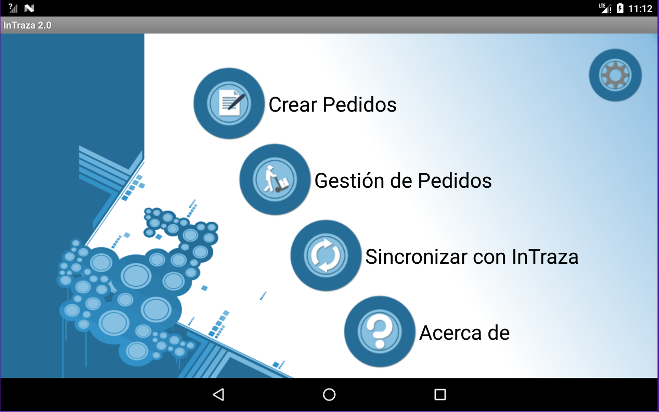
\includegraphics[width=0.65\linewidth]{figuras/manual/p1}
	\caption{Intraza - pantalla principal}
	\label{fig:Itzp1}
\end{figure}

\subsection{Creación de pedidos}

En esta pantalla elegiremos el cliente por medio del combo, además de la fecha de entrega y observaciones del pedido. Las observaciones pueden dictarse, escribirse o elegirse de una lista predefinida para ese cliente. Cuando seleccionas fijar observaciones añades estas a la lista de observaciones prefijadas. 

\begin{figure}[H]
	\centering
	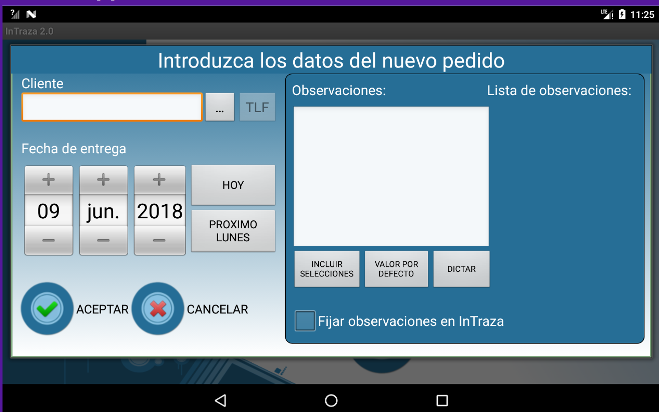
\includegraphics[width=0.65\linewidth]{figuras/manual/p3}
	\caption{Intraza - creación de pedidos}
	\label{fig:Itzp2}
\end{figure}

Una vez validada la pantalla anterior, nos muestra una pantalla a la que llamaremos ruteros que muestra las lineas de pedido de la empresa seleccionada y nos permite crear adicionales. Podremos mostrar/ocultar las lineas antiguas y volver a la pantalla anterior si queremos cambiar algo, por medio de los botones. Ademas podremos sincronizar los ruteros de la empresa seleccionada.

\begin{figure}[H]
	\centering
	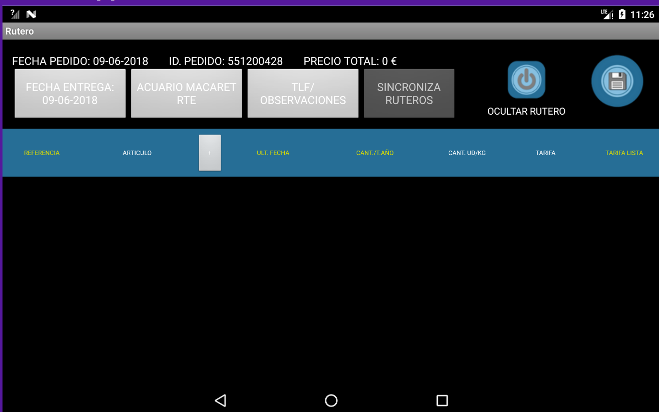
\includegraphics[width=0.65\linewidth]{figuras/manual/p2}
	\caption{Intraza - ruteros}
	\label{fig:Itzp3}
\end{figure}

\pagebreak

Una vez pulsado el botón de añadir artículo '(+)' nos mostrará un ventana de dialogo para elegir el artículo que queremos introducir. 

\begin{figure}[H]
	\centering
	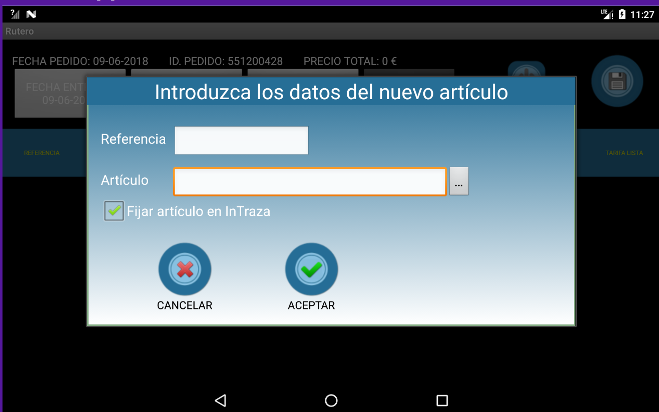
\includegraphics[width=0.7\linewidth]{figuras/manual/p4}
	\caption{Intraza - introducir articulo}
	\label{fig:Itzp4}
\end{figure}

Una vez aceptado el articulo nos mostrará la pantalla para rellenar los campos necesarios para el pedido. Ademas nos permitirá clonar un rutero para pedidos repetitivos.

\begin{figure}[H]
	\centering
	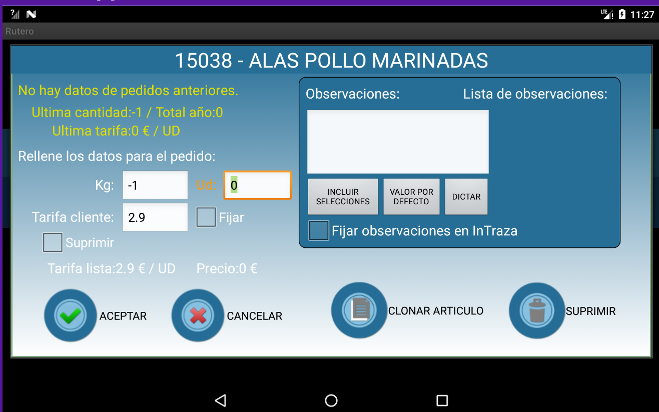
\includegraphics[width=0.7\linewidth]{figuras/manual/p5}
	\caption{Intraza - rellenar cantidades/observaciones}
	\label{fig:Itzp5}
\end{figure}

\pagebreak
Una ver añadido el articulo podemos comprobar que la pantalla ruteros dispone de una linea con los datos del mismo.

\begin{figure}[H]
	\centering
	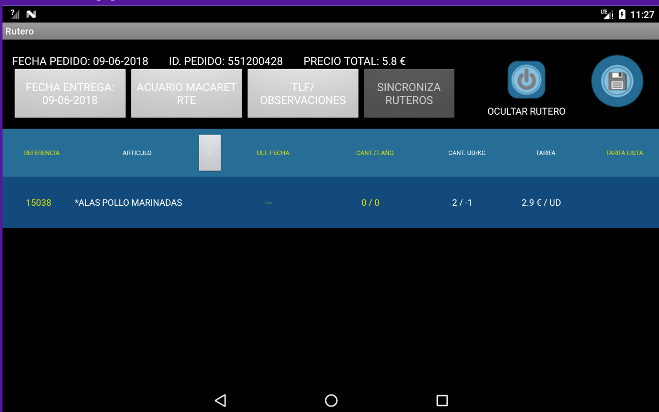
\includegraphics[width=0.7\linewidth]{figuras/manual/p6}
	\caption{Intraza - articulo insertado}
	\label{fig:Itzp6}
\end{figure}

\subsection{Gestión de pedidos}

En esta pantalla podremos elegir todos los pedidos o elegir los pedidos del cliente que queremos visualizar.

\begin{figure}[H]
	\centering
	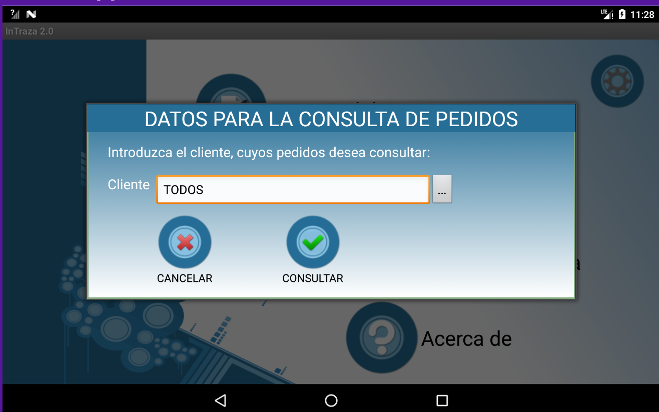
\includegraphics[width=0.7\linewidth]{figuras/manual/p7}
	\caption{Intraza - gestión de pedidos}
	\label{fig:Itzp7}
\end{figure}

\pagebreak
En esta pantalla podremos gestionar los pre-pedidos que están almacenados en el dispositivo. Podremos ver su contenido clickando en el id de pedido. Ademas podremos borrarlos o enviarlos a la central, para que pasen a ser parte del ERP.

\begin{figure}[H]
	\centering
	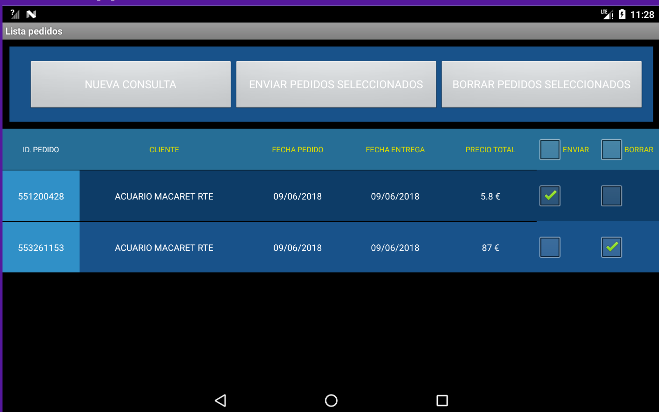
\includegraphics[width=0.7\linewidth]{figuras/manual/p9}
	\caption{Intraza - lista de pedidos}
	\label{fig:Itzp8}
\end{figure}

\subsection{Sincronizar con Intraza}

Por medio de esta pantalla podremos sincronizar los datos guardados en el ERP, con los datos de la aplicación. Sincronizará clientes, artículos y ruteros.

\begin{figure}[H]
	\centering
	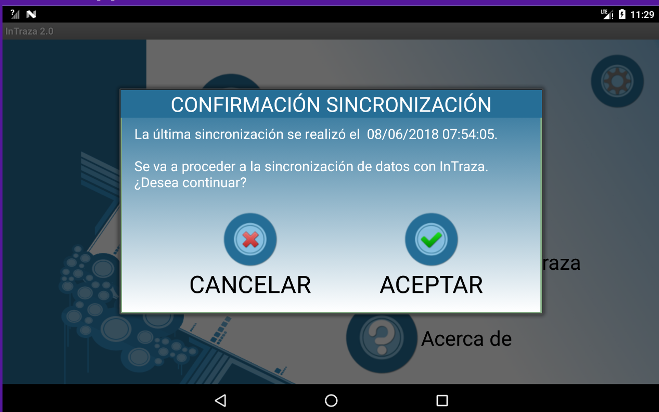
\includegraphics[width=0.7\linewidth]{figuras/manual/p10}
	\caption{Intraza - sincronización}
	\label{fig:Itzp9}
\end{figure}

\subsection{Configuración}

En esta pantalla podremos configurar el valor de algunos parámetros de la aplicación. Como por ejemplo la ruta del WebService de comunicaciones. Esta pantalla está protegida con contraseña.

\begin{figure}[H]
	\centering
	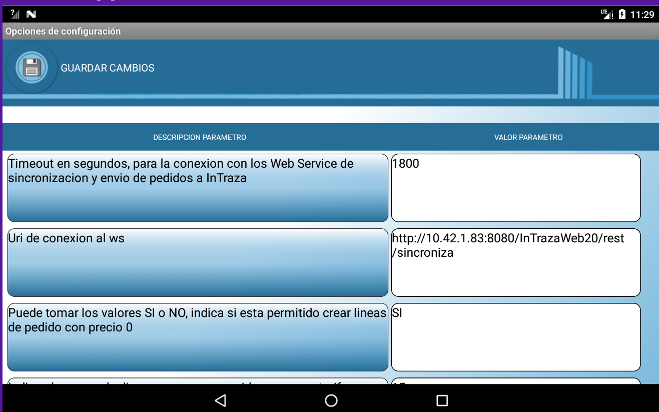
\includegraphics[width=0.7\linewidth]{figuras/manual/p8}
	\caption{Intraza - configuración}
	\label{fig:Itzp10}
\end{figure}

